\documentclass[aspectratio=169]{beamer}
\usepackage{fontawesome} % Required for FontAwesome icons
\usepackage{graphicx,ualberta,url}
\usepackage[english]{babel}
\usepackage[latin1]{inputenc}
%\usepackage{times}
\usepackage[T1]{fontenc}
\usepackage{multirow}
\usepackage{capt-of}
\usepackage{graphicx}
\usepackage{array}
\usepackage{tikz}
\usepackage{ifpdf}

\urlstyle{same}

\hypersetup{
    colorlinks,
    citecolor= blue,
    filecolor= blue,
    linkcolor= ualbertagold,
    urlcolor= ualbertagreen
}

\newcommand{\TextUnderscore}{\rule{.4em}{.4pt}}

\newcommand*{\vcenteredhbox}[1]{\begingroup
\setbox0=\hbox{#1}\parbox{\wd0}{\box0}\endgroup}

\newcommand{\icon}[4][black]{% The first parameter is the FontAwesome icon name, the second is the box size and the third is the text
    \vcenteredhbox{{
    \makebox(#3, #3){\textcolor{#1}{\large\csname fa#2\endcsname}}
    }}% Icon and box
	\hspace{0.2cm}% Whitespace
    \vcenteredhbox{
    \textcolor{#1}{#4}
    }% Text
}

%----------------------------------------------------------------------------------------
%	GRAPHICS DEFINITIONS
%----------------------------------------------------------------------------------------

\definecolor{bg-color}{HTML}{4b6a78}
\definecolor{grayish}{HTML}{DDDDDD}
\definecolor{code}{HTML}{e83e8c}


\begin{document}

\title[Carbon Price Pass-Through]{Carbon Price Pass-Through in Alberta's Electricity Market}
%\author{Branko Bo\v skovi\'{c} \and Andrew Leach \and Charles F.\ Mason}
%\institute{University of Alberta  \and University of Alberta  \and University of Wyoming}

%\author[shortname]{author1 \inst{1} \and author2 \inst{2}}
%\institute[shortinst]{\inst{1} affiliation for author1 \and %
 %                     \inst{2} affiliation for author2}

\author[Leach and Shaffer]{%
  \texorpdfstring{%
    \begin{columns}
      \column{.1\linewidth}
      \column{.4\linewidth}
      \centering
      Andrew Leach \\University of Alberta
      \column{.4\linewidth}
      \centering
      Blake Shaffer \\University of Calgary
      \column{.1\linewidth}
      \end{columns}
 }
 {Leach and Shaffer (2022)}
}
\date{CEA Conference 2022}

%\frame[plain]{
%  \titlepage
%}

\frame{\vspace{-2cm}
  \titlepage
}



\section{Introduction}

\begin{frame}{Carbon Pricing's Effect on Electricity Markets}
    \begin{itemize}
    \item We want to understand how firms react to carbon pricing: do they pass through marginal prices as our models assume?
    \item Electricity markets are a real-life supply and demand model
    \item Alberta GHG policies changed carbon prices and output-based credit allocations across time and facilities
    \item We build a rich data set of relevant firm and market covariates
    \item Our results show weaker pass through than seen in Fabra and Reguant (2014) or Hintermann (2016) which each find near-complete pass-through of emissions costs
    \item We are left with the question of why costs might not be fully passed-through to market offer curves, at least for marginal blocks of power
    \end{itemize}
\vfill
\end{frame}


\section{Motivation and Context}

%\begin{frame}{Oil sands reserves\hspace{3cm} \small Source: AER (2013)}
%\pgfputat{\pgfxy(0,.25)}{\pgfimage[width=4.25in]{AB_reserves.pdf}}
%\end{frame}

\begin{frame}{Alberta's Power Market is an Ideal Laboratory}
    \begin{itemize}
    \item Alberta's power market is relatively small, isolated, with minimal intertie capacity:
    \small\begin{itemize}
    \item WECC (1325 MW export and 1500 MW import) and Saskatchewan (150 MW)
        \end{itemize}
    \end{itemize}
\vfill
\end{frame}

\begin{frame}{Alberta Power Market}
   \tikz [remember picture,overlay]
    \node[yshift=-.85cm,xshift=0cm] at (current page.center)
       {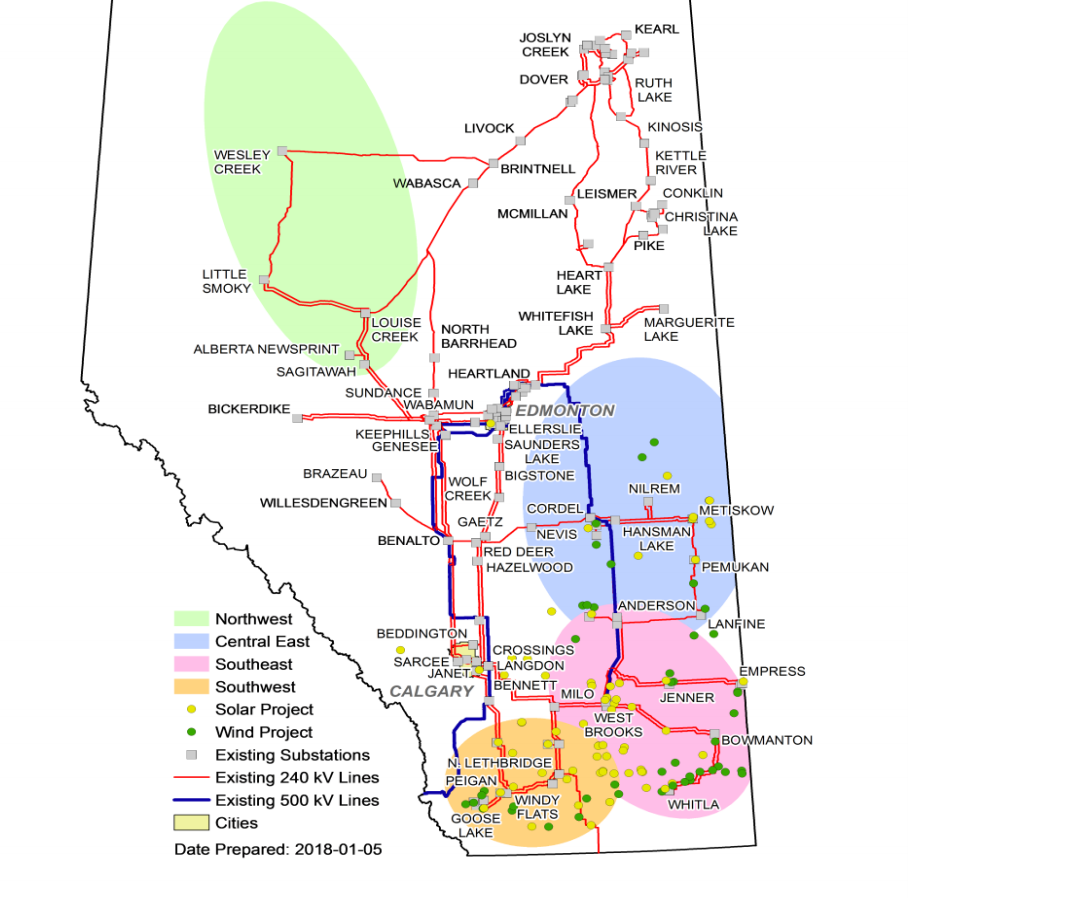
\includegraphics[width=.5\paperwidth]{../images/alberta_grid.png}}; \vspace{1cm}
   \vfill
\end{frame}

\begin{frame}{Alberta's Power Market is an Ideal Laboratory}
    \begin{itemize}
    \item Alberta's power market is relatively small, isolated, with minimal intertie capacity:
    \small\begin{itemize}
    \item WECC (1325 MW export and 1500 MW import) and Saskatchewan (150 MW)
        \end{itemize}
    \item Alberta's market is winter-peaking (load) but often has high summer prices
  \end{itemize}
\vfill
\end{frame}


\begin{frame}{Alberta Power Market Prices and Loads}
   \tikz [remember picture,overlay]
    \node[yshift=-0.6cm,xshift=0cm] at (current page.center)
       {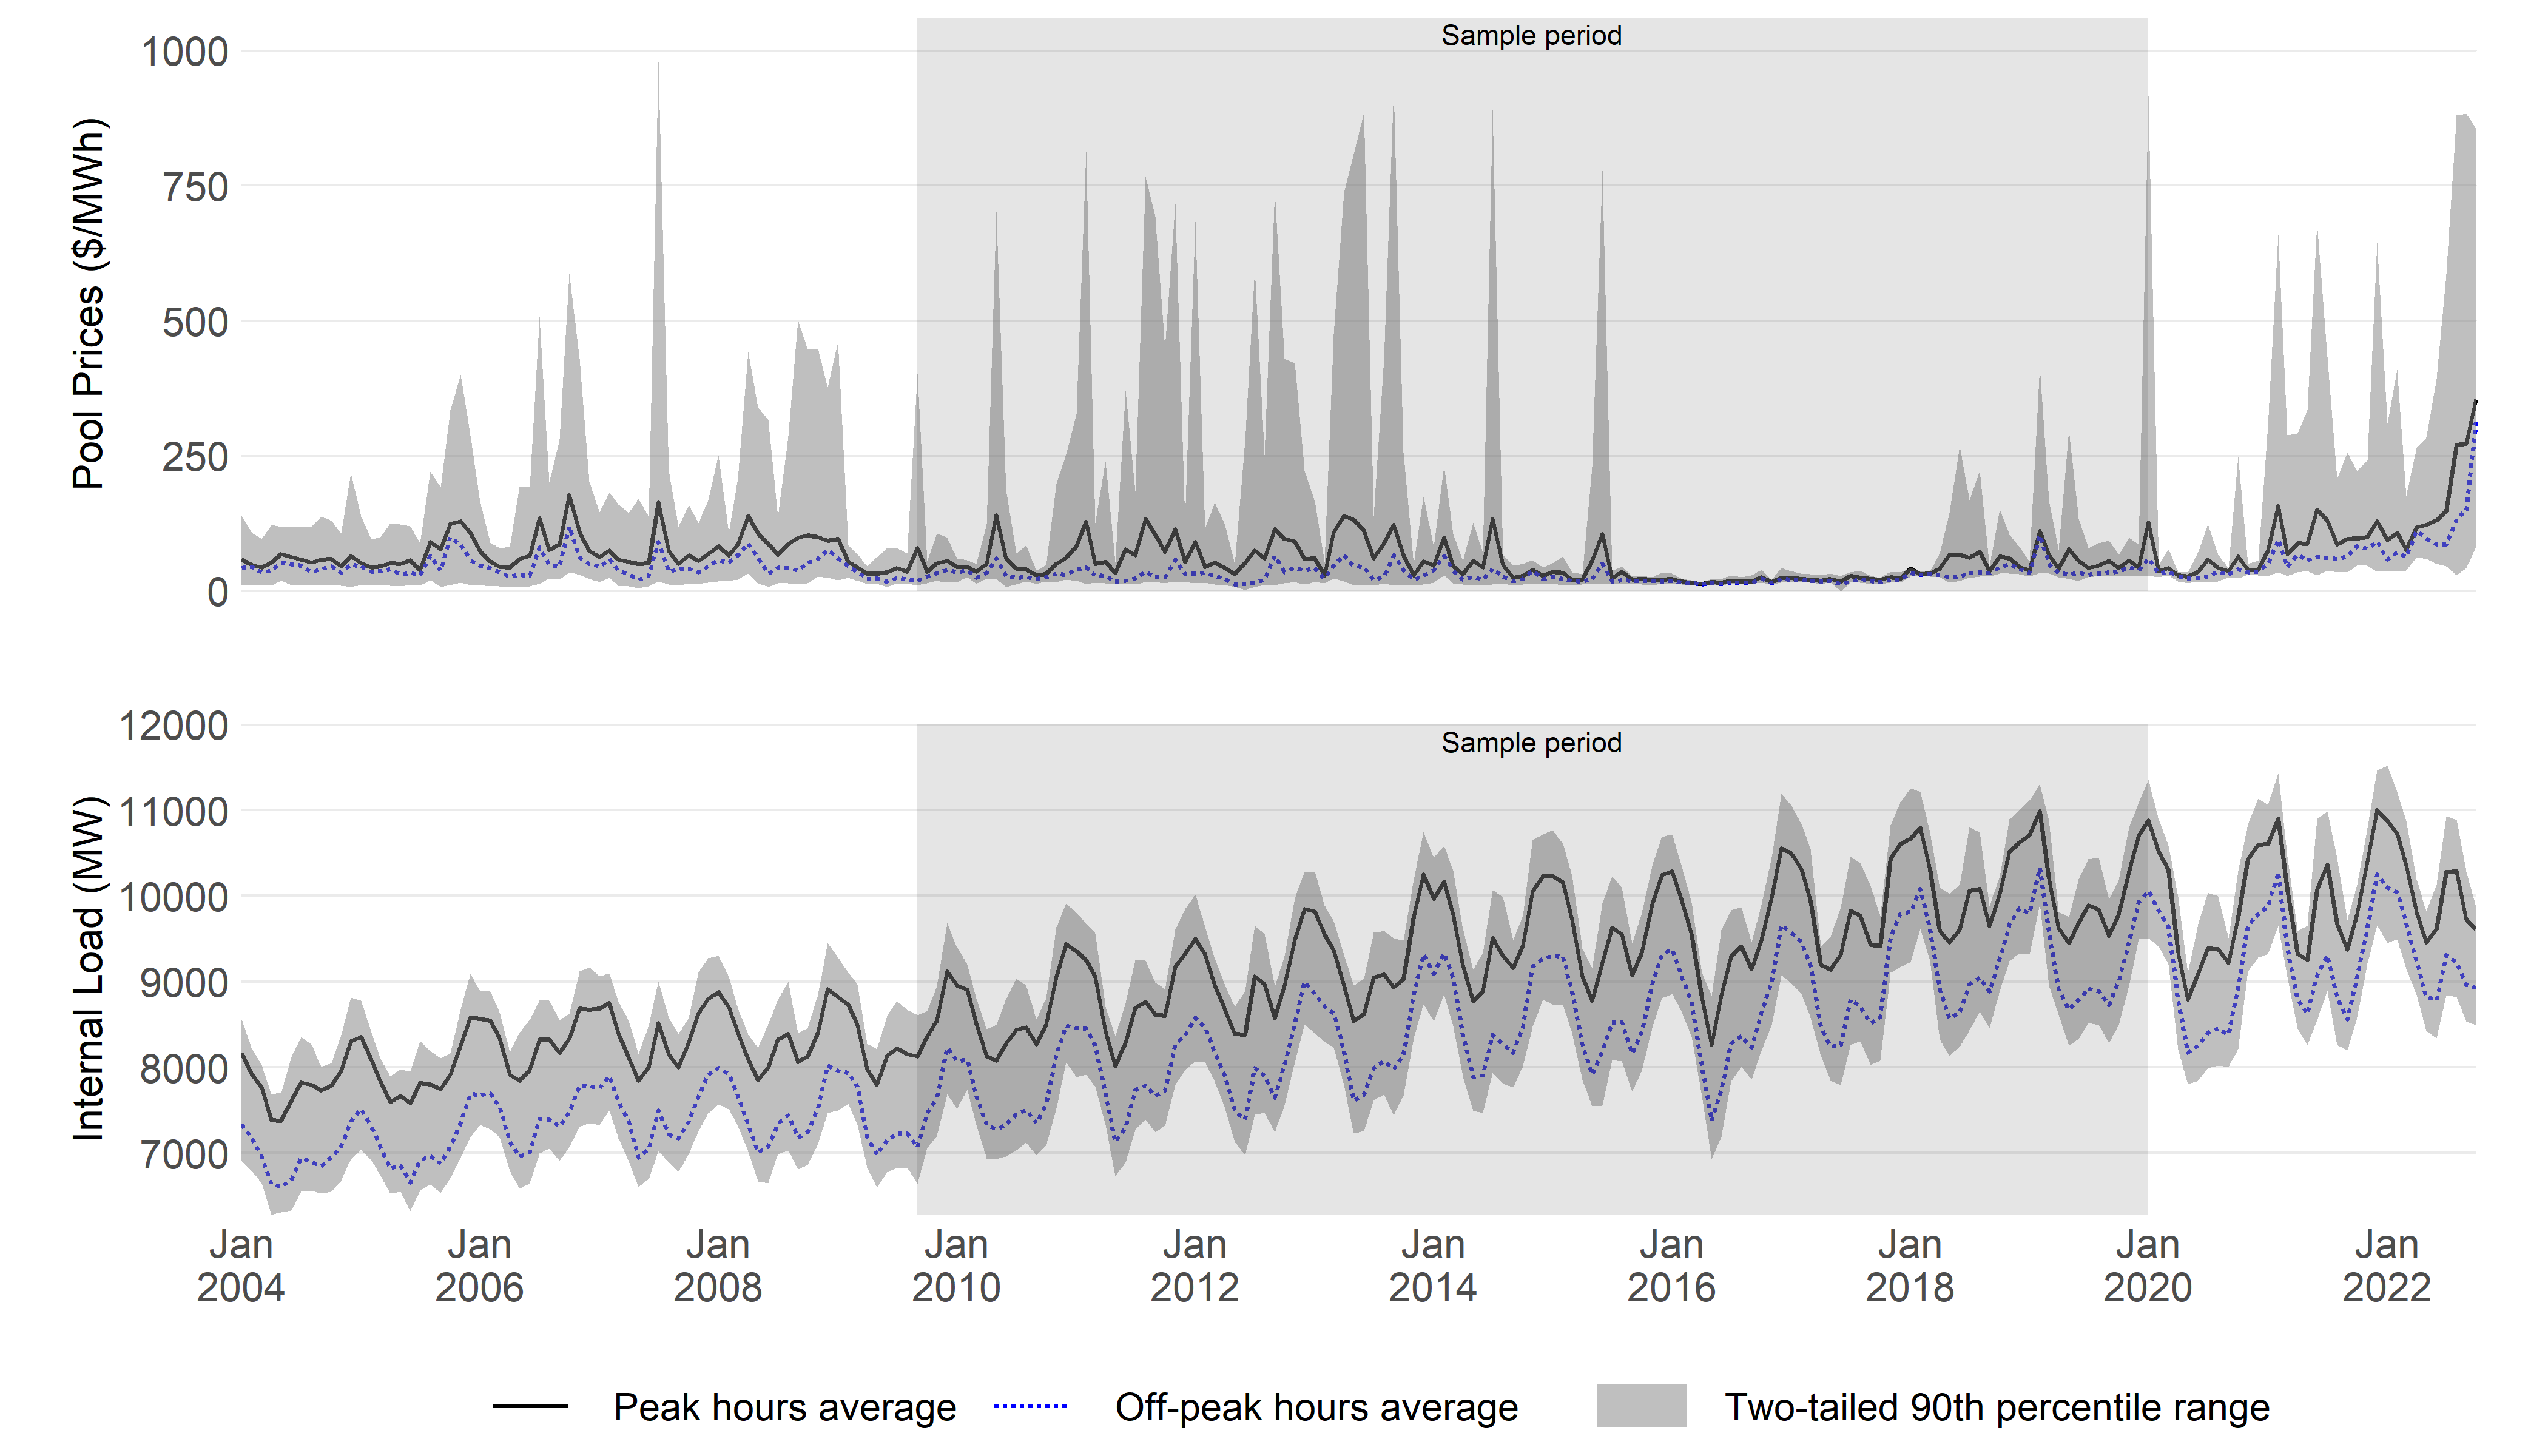
\includegraphics[width=.75\paperwidth]{../images/prices_and_loads.png}}; \vspace{1cm}
   \vfill
\end{frame}


\begin{frame}{Alberta's Power Market is an Ideal Laboratory}
    \begin{itemize}
    \item Alberta's power market is relatively small, isolated, with minimal intertie capacity:
    \small\begin{itemize}
    \item WECC (1325 MW export and 1500 MW import) and Saskatchewan (150 MW)
        \end{itemize}
    \item Alberta's market is winter-peaking (load) but often has high summer prices
    \item Alberta's market has a wide variety of sources of generation
  \end{itemize}
\vfill
\end{frame}

\begin{frame}{Alberta Power Generation Sources}
   \tikz [remember picture,overlay]
    \node[yshift=-0.6cm,xshift=0cm] at (current page.center)
       {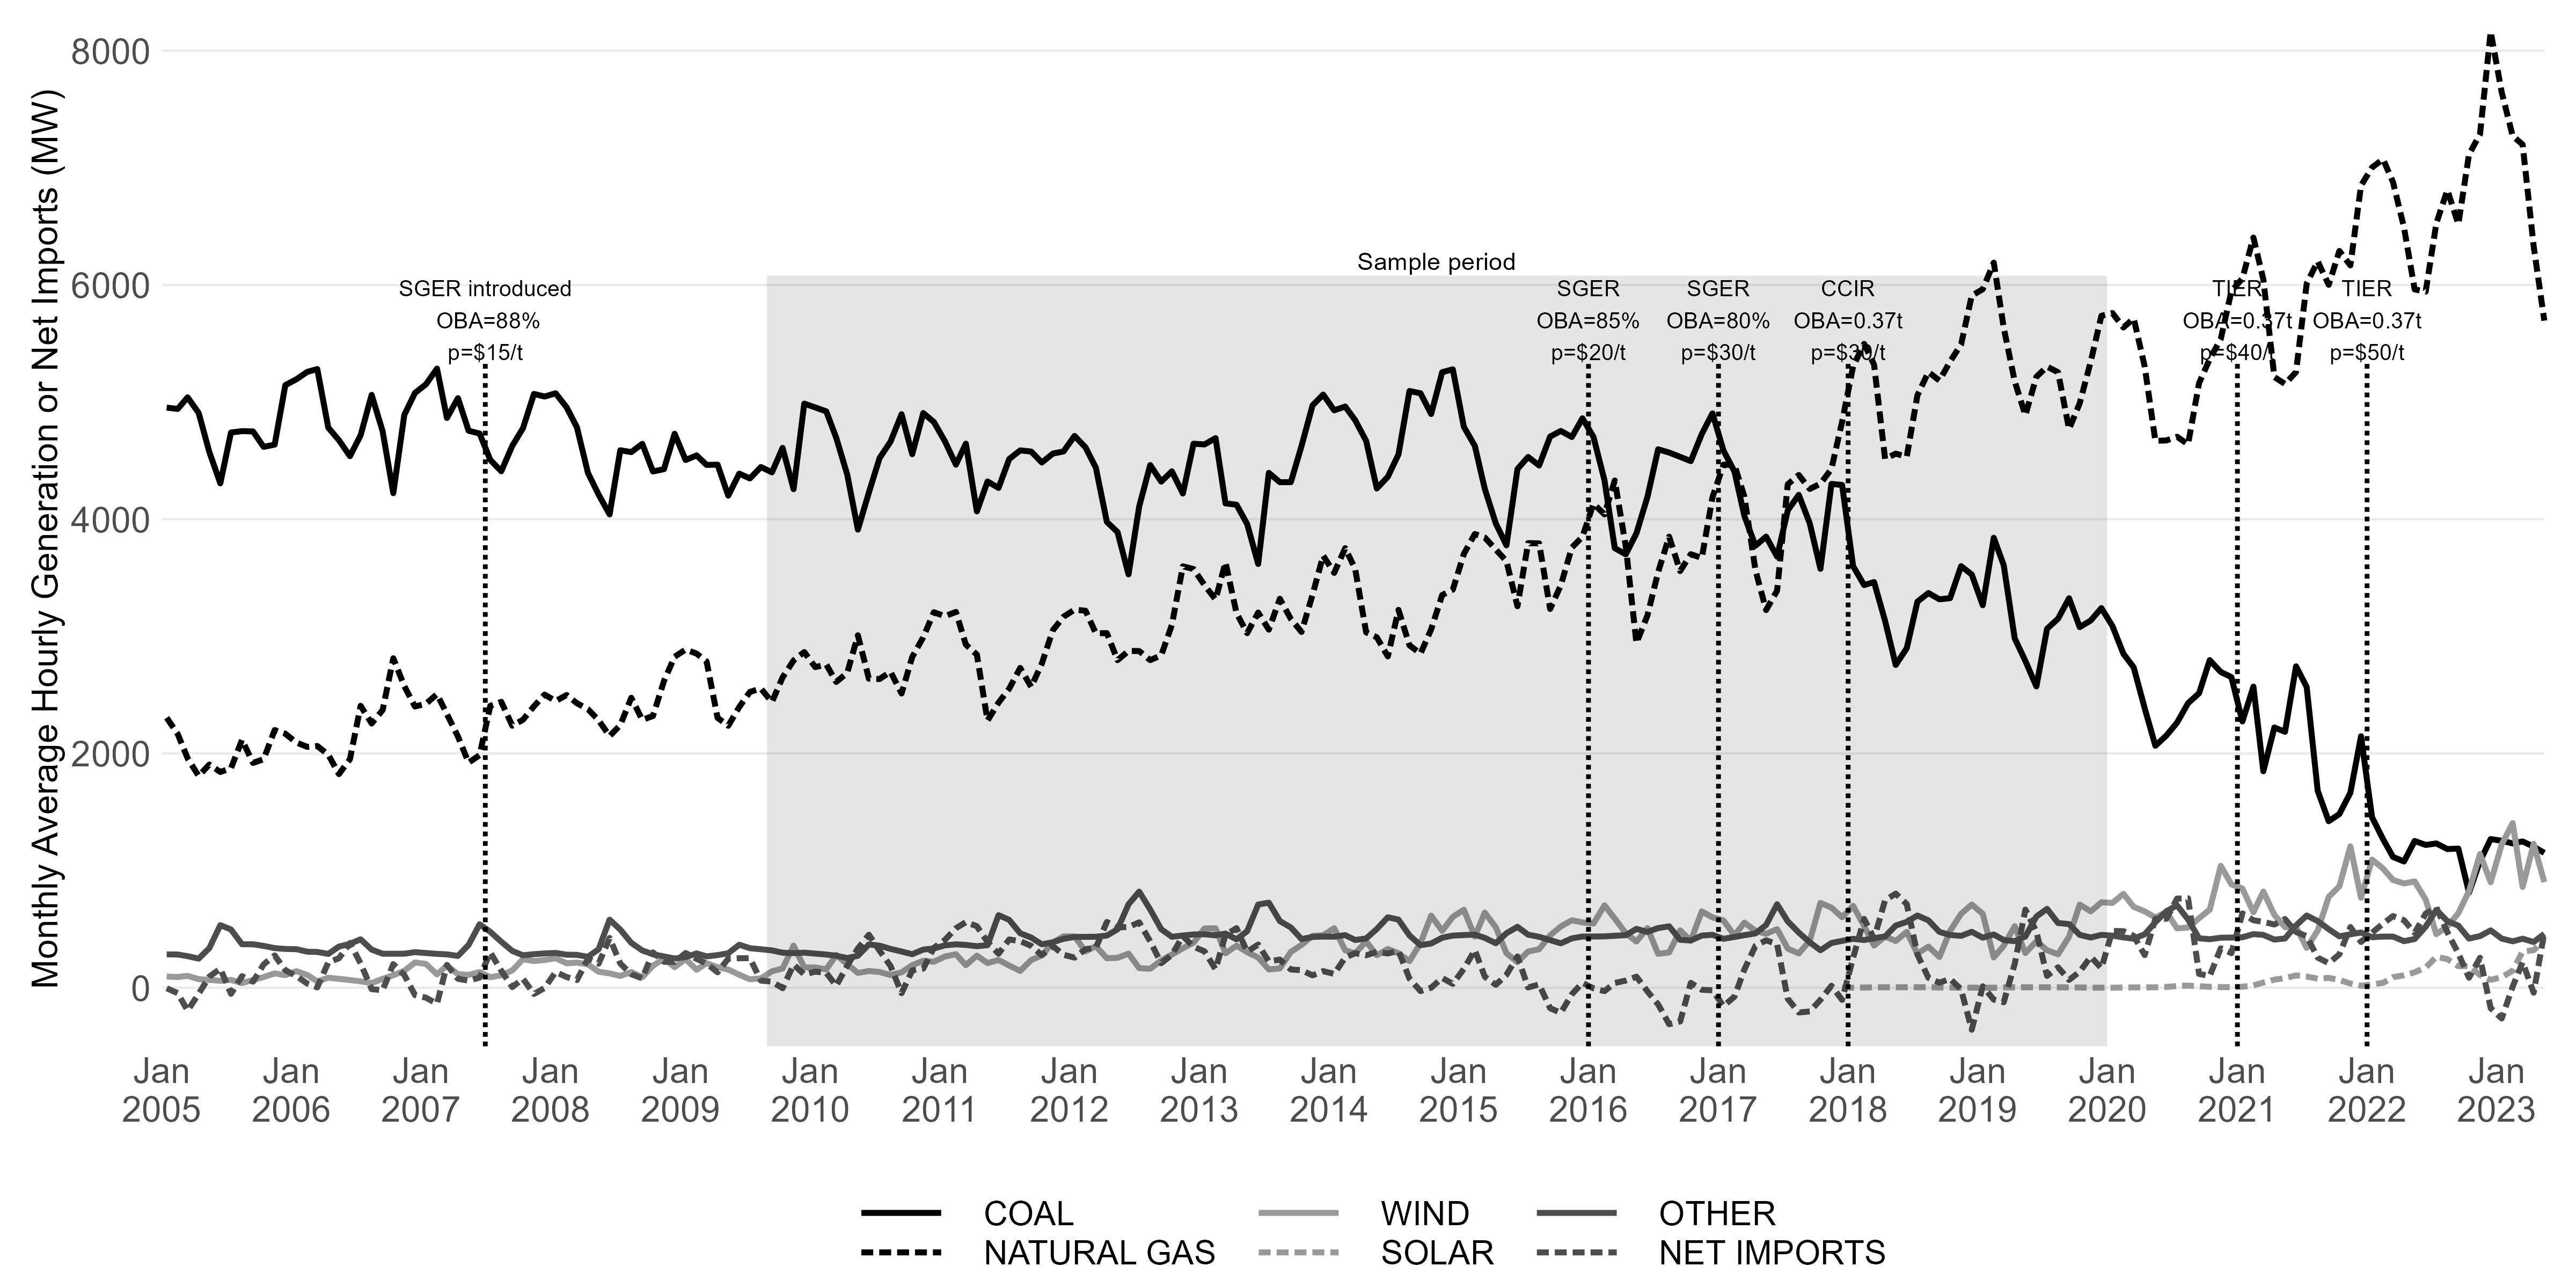
\includegraphics[width=.85\paperwidth]{../images/gen_fuel_policies.png}}; \vspace{1cm}
   \vfill
\end{frame}

\begin{frame}{Alberta's Power Market is an Ideal Laboratory}
    \begin{itemize}
    \item Alberta's power market is relatively small, isolated, with minimal intertie capacity:
    \small\begin{itemize}
    \item WECC (1325 MW export and 1500 MW import) and Saskatchewan (150 MW)
        \end{itemize}
    \item Alberta's market is winter-peaking (load) but often has high summer prices
    \item Alberta's market has a wide variety of sources of generation
    \item Carbon emissions reporting covers most facilities in the market
    \small\begin{itemize}
    \item Carbon pricing has been in place since 2007
    \item Carbon pricing design changed repeatedly from 2015-2022
        \end{itemize}
  \end{itemize}
\vfill
\end{frame}


\begin{frame}{Alberta's Policy Changes as Treatments}
    \begin{itemize}
    \item 2007-2015: \textit{Specified Gas Emitters Regulation (SGER)}
    \small\begin{itemize}
    \item Price of \$15/t, OBAs at 88\% of historic GHG/MWh
    \item Covered only large (>100kt/yr) facilities
    \end{itemize}
    \item 2016-2017: \textit{Specified Gas Emitters Regulation (SGER)}
    \small\begin{itemize}
    \item 2016: price \$20/t, OBAs at 85\% of historic GHG/MWh
    \item 2017: price \$30/t, OBAs at 80\% of historic GHG/MWh
    \item Covered only large (>100kt/yr) facilities
    \end{itemize}
    \item 2018-2019: \textit{Carbon Competitiveness Incentive Regulation (CCIR)}
    \small\begin{itemize}
    \item 2018-19: price \$30/t, OBAs at 0.37t/MWh for all facilities
    \item Covered large (>100kt/yr) facilities, with opt-in provision
    \end{itemize}
    \item 2019-present: \textit{Technology Innovation and Emissions Reduction Regulation (TIER)}
    \small\begin{itemize}
    \item 2020: price \$30/t, OBAs at 0.37t/MWh for all facilities
    \item 2021: price \$40/t, OBAs at 0.37t/MWh for all facilities
    \item 2022: price \$50/t, OBAs at 0.37t/MWh for all facilities
    \item Covers large (>100kt/yr) facilities, with opt-in provision
    \end{itemize}
    \end{itemize}
\vfill
\end{frame}

\begin{frame}{Carbon pricing impacts across facilities over time}
    \tikz [remember picture,overlay]
    \node[yshift=-.1cm,xshift=0cm] at (current page.center)
       {\includegraphics[width=.85\paperwidth]{../../sger/compliance_cost_policies.png}}; \vspace{4.85cm}
   \begin{itemize}
    \item different impacts of carbon pricing on plants of the same type at the same time, and changes in pricing for the same plants over time combine to allow us to identify expected pass-through of carbon tax costs and OBA value
    \end{itemize}
   \vfill
\end{frame}

\section{Empirical Framework}
\begin{frame}{Empirical Framework}
    \begin{itemize}
    \item We estimate GHG cost pass through using samples drawn from merit orders at each hour $t$ at each of $J$ percentile support points to estimate:
    \small\begin{align*}\label{eq:regression}
 \underbrace{P_{j,t}}_{\substack{\text{Offer value} \\ \text{at percentile }j\\ \text{at time }t}}&=
 \underbrace{\alpha_{j}}_{\substack{\text{Constant for} \\ \text{percentile }j}}+
 \underbrace{\beta_j M_t}_{\substack{\text{Market, policy, and} \\ \text{climate variables} \\\text{at time }t}}+
 \underbrace{\delta_j F_{j,t}}_{\substack{\text{Facility} \\ \text{characteristics} \\ \text{at percentile }j\\ \text{at time }t}}+\\&
 \underbrace{\zeta_j t_{j,t}}_{\substack{\text{Carbon cost} \\ \text{at percentile j}\\ \text{at time }t}}+
 \underbrace{\kappa_j O_{j,t}}_{\substack{\text{OBA value} \\ \text{at percentile j}\\ \text{at time }t}}+
 \underbrace{\epsilon_{j,t}}_{\substack{\text{Error term}}}
\end{align*}
     \end{itemize}
   \vfill
\end{frame}

\begin{frame}{Empirical Framework}
       \tikz [remember picture,overlay]
    \node[yshift=-.7cm,xshift=0cm] at (current page.center)
       {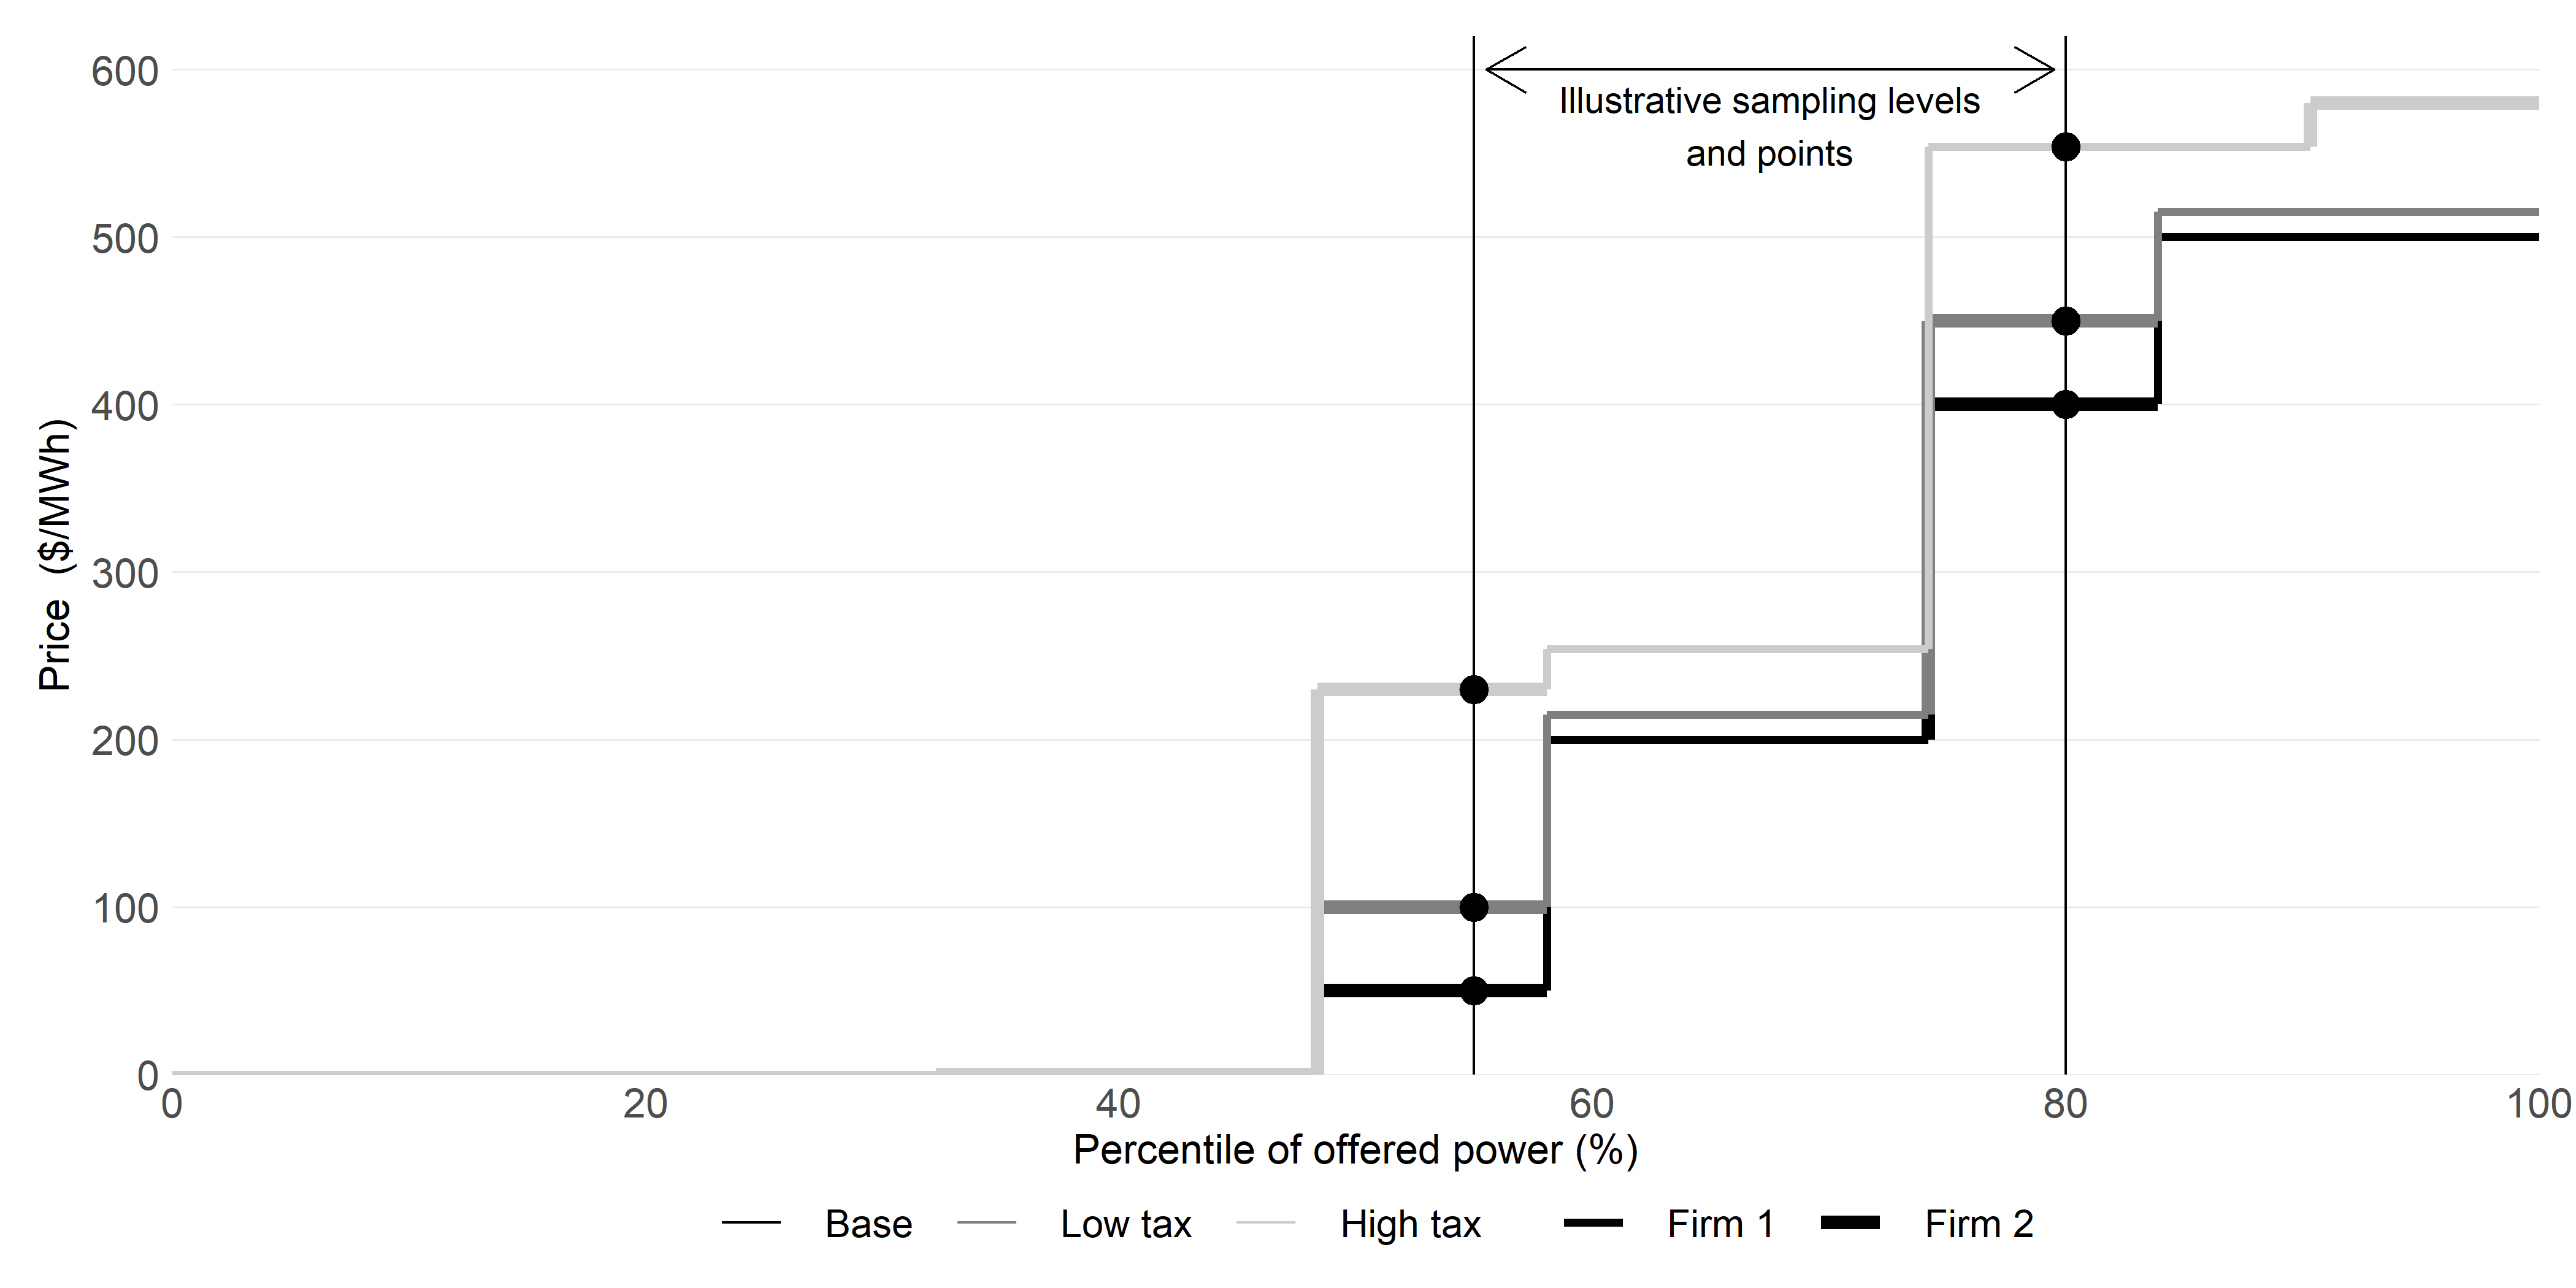
\includegraphics[width=.8\paperwidth]{../images/sampling.png}}; \vspace{1cm}
   \vfill
\end{frame}


\begin{frame}{Empirical Framework}
       \tikz [remember picture,overlay]
    \node[yshift=-.7cm,xshift=0cm] at (current page.center)
       {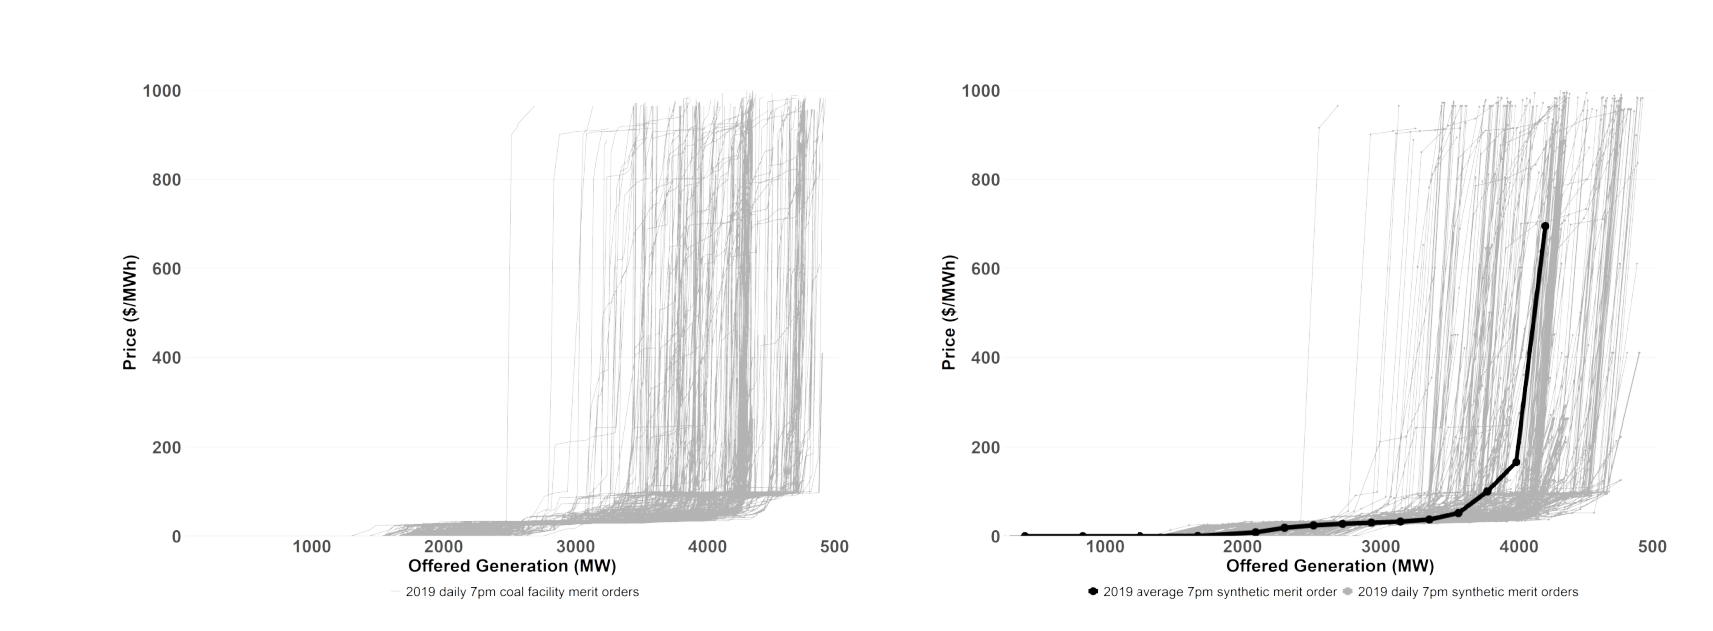
\includegraphics[width=.99\paperwidth]{../images/coal_synth_cea.png}}; \vspace{1cm}
   \vfill
\end{frame}

\begin{frame}{Empirical Framework}
    \begin{itemize}
    \item We estimate GHG cost pass through using samples drawn from merit orders at each hour $t$ at each of $J$ percentile support points to estimate:
    \small\begin{align*}
 \underbrace{P_{j,t}}_{\substack{\text{Offer value} \\ \text{at percentile }j\\ \text{at time }t}}&=
 \underbrace{\alpha_{j}}_{\substack{\text{Constant for} \\ \text{percentile }j}}+
 \underbrace{\beta_j M_t}_{\substack{\text{Market, policy, and} \\ \text{climate variables} \\\text{at time }t}}+
 \underbrace{\delta_j F_{j,t}}_{\substack{\text{Facility} \\ \text{characteristics} \\ \text{at percentile }j\\ \text{at time }t}}+\\&
 \underbrace{\zeta_j t_{j,t}}_{\substack{\text{Carbon cost} \\ \text{at percentile j}\\ \text{at time }t}}+
 \underbrace{\kappa_j O_{j,t}}_{\substack{\text{OBA value} \\ \text{at percentile j}\\ \text{at time }t}}+
 \underbrace{\epsilon_{j,t}}_{\substack{\text{Error term}}}
\end{align*}
\item The estimated values of parameters $\zeta_j$ and $\kappa_j$ will tell us the degree of pass-through of carbon tax costs and OBA values at each percentile $j$ of each merit order we examine.
     \end{itemize}
   \vfill
\end{frame}

\begin{frame}{Expected Estimates of  $\zeta_j$}
       \tikz [remember picture,overlay]
    \node[yshift=-.6cm,xshift=0cm] at (current page.center)
       {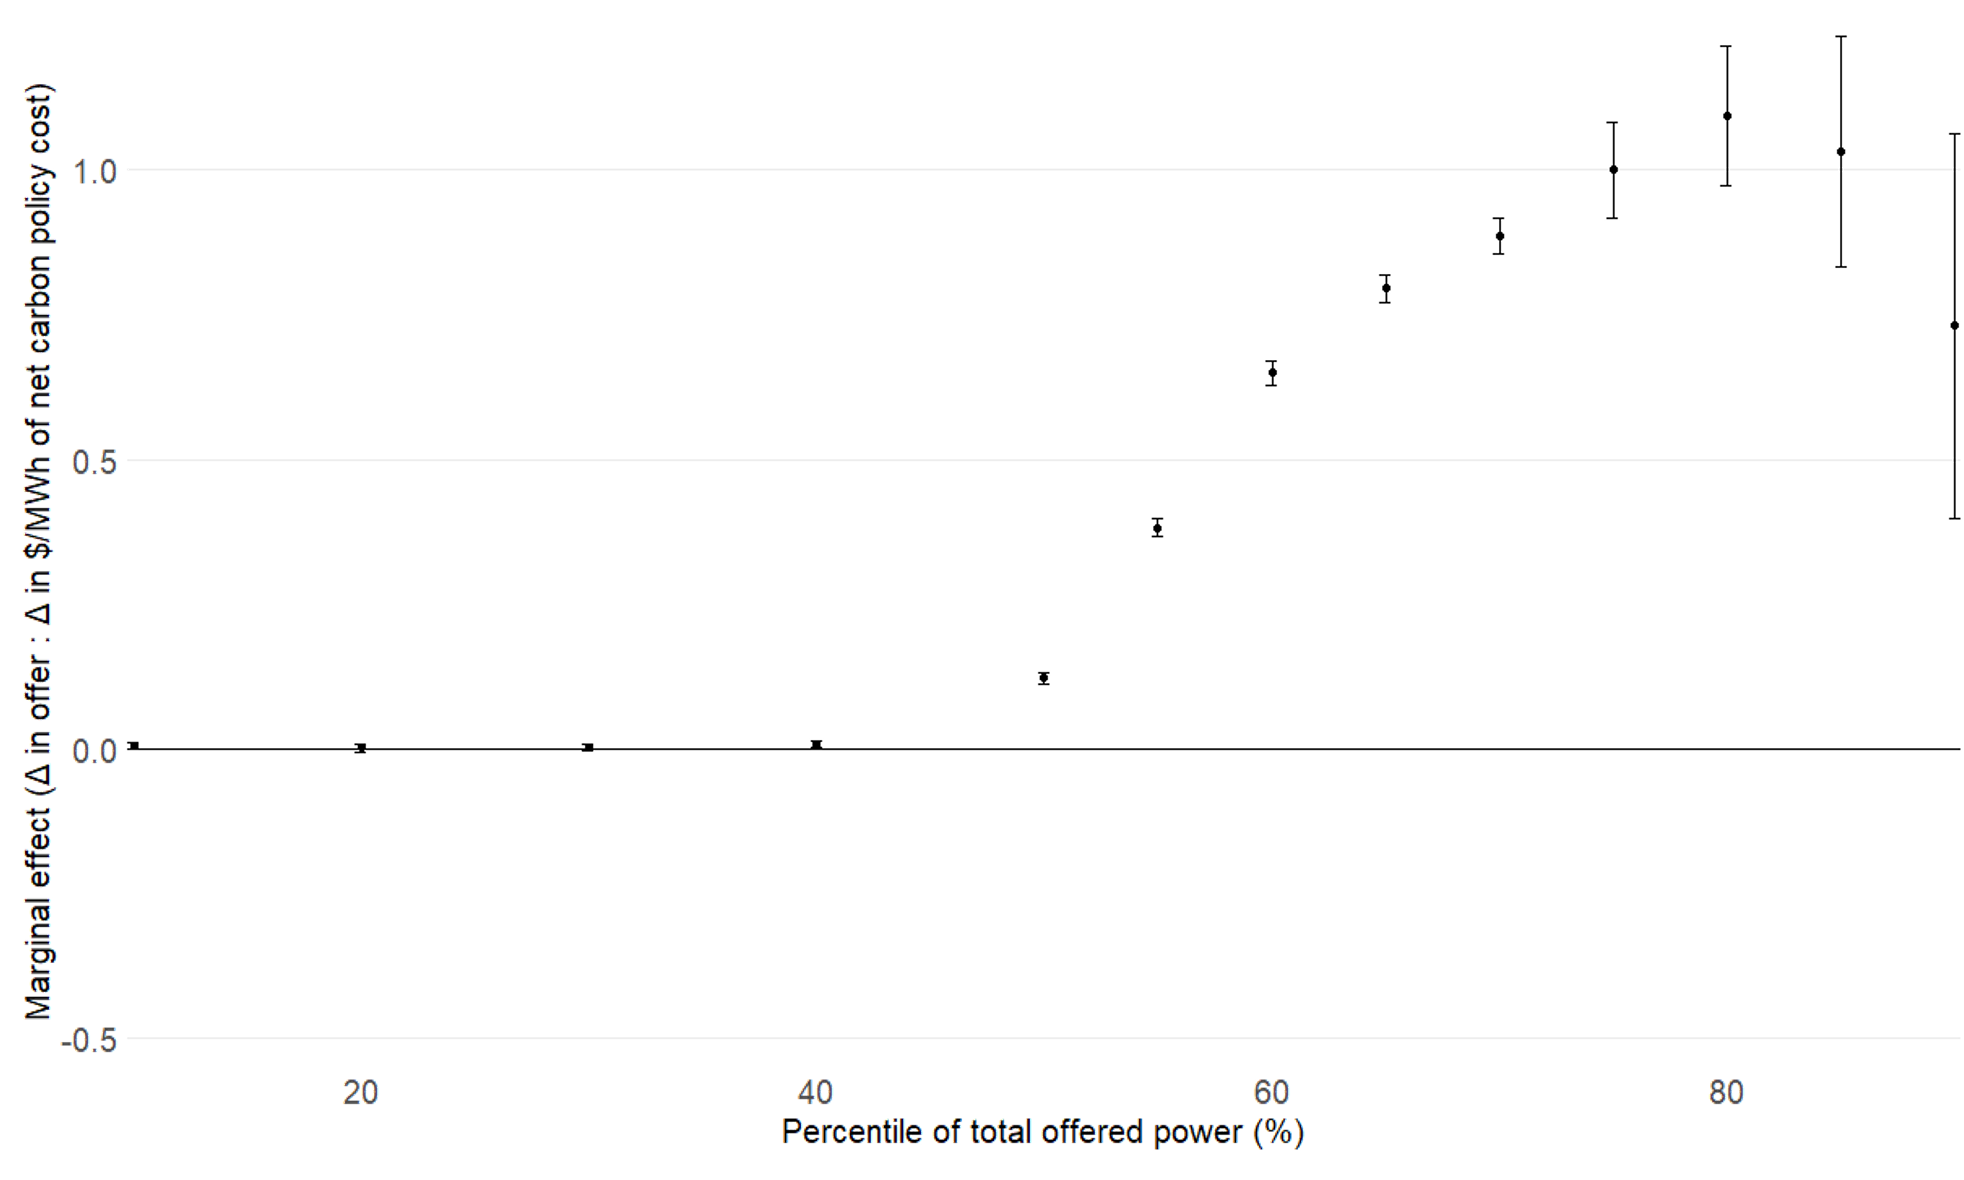
\includegraphics[width=.7\paperwidth]{../images/expectation.png}}; \vspace{1cm}
   \vfill
\end{frame}



\section{Results}

\begin{frame}{Carbon pricing pass through, full market}
   \tikz [remember picture,overlay]
    \node[yshift=-.6cm,xshift=0cm] at (current page.center)
        {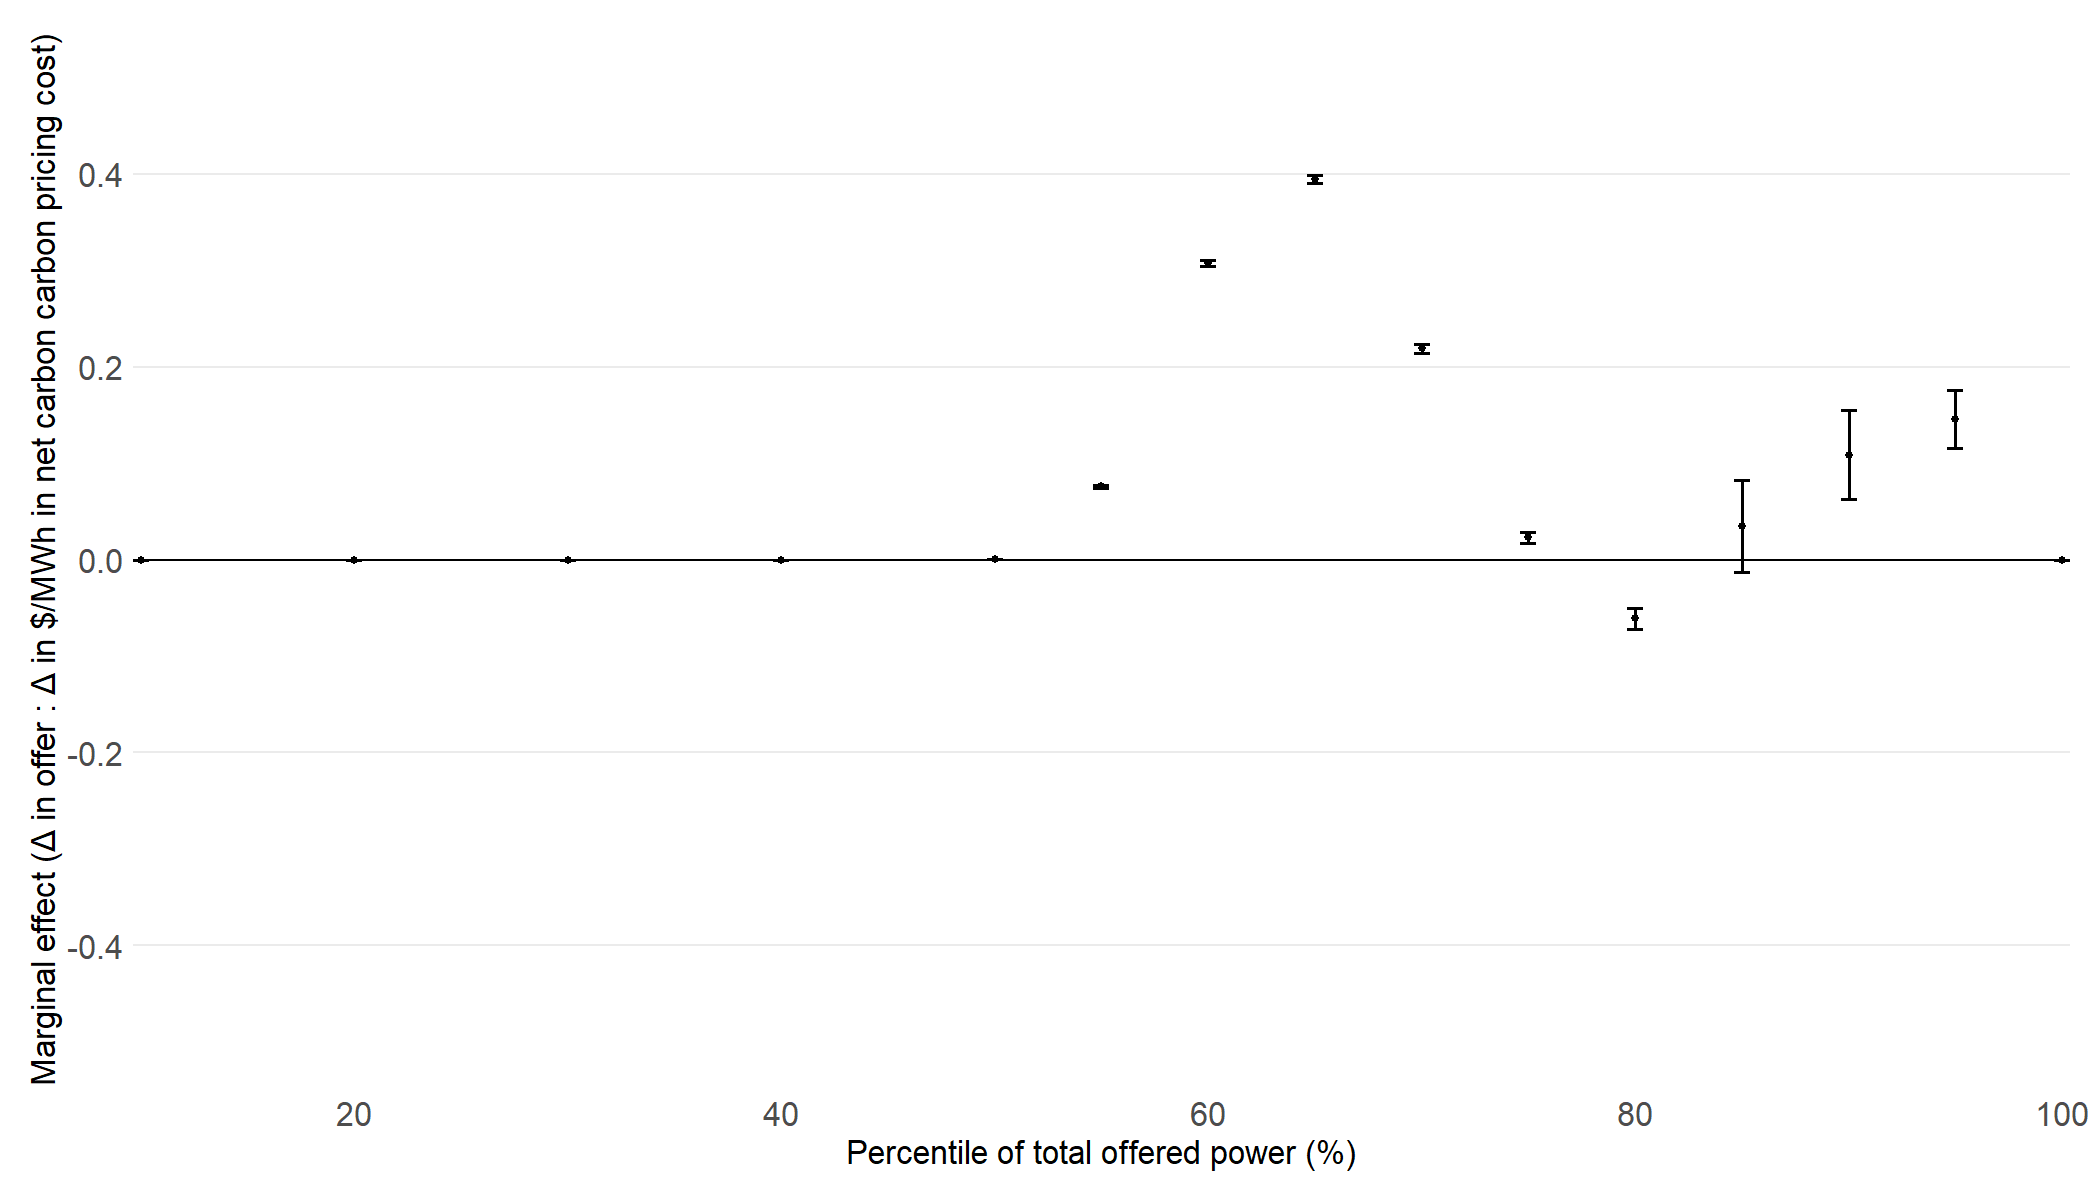
\includegraphics[width=.7\paperwidth]{../images/all_plants_net.png}}; \vspace{1cm}
   \vfill
\end{frame}

\begin{frame}{Carbon pricing pass through, full market}
   \tikz [remember picture,overlay]
    \node[yshift=-.6cm,xshift=0cm] at (current page.center)
        {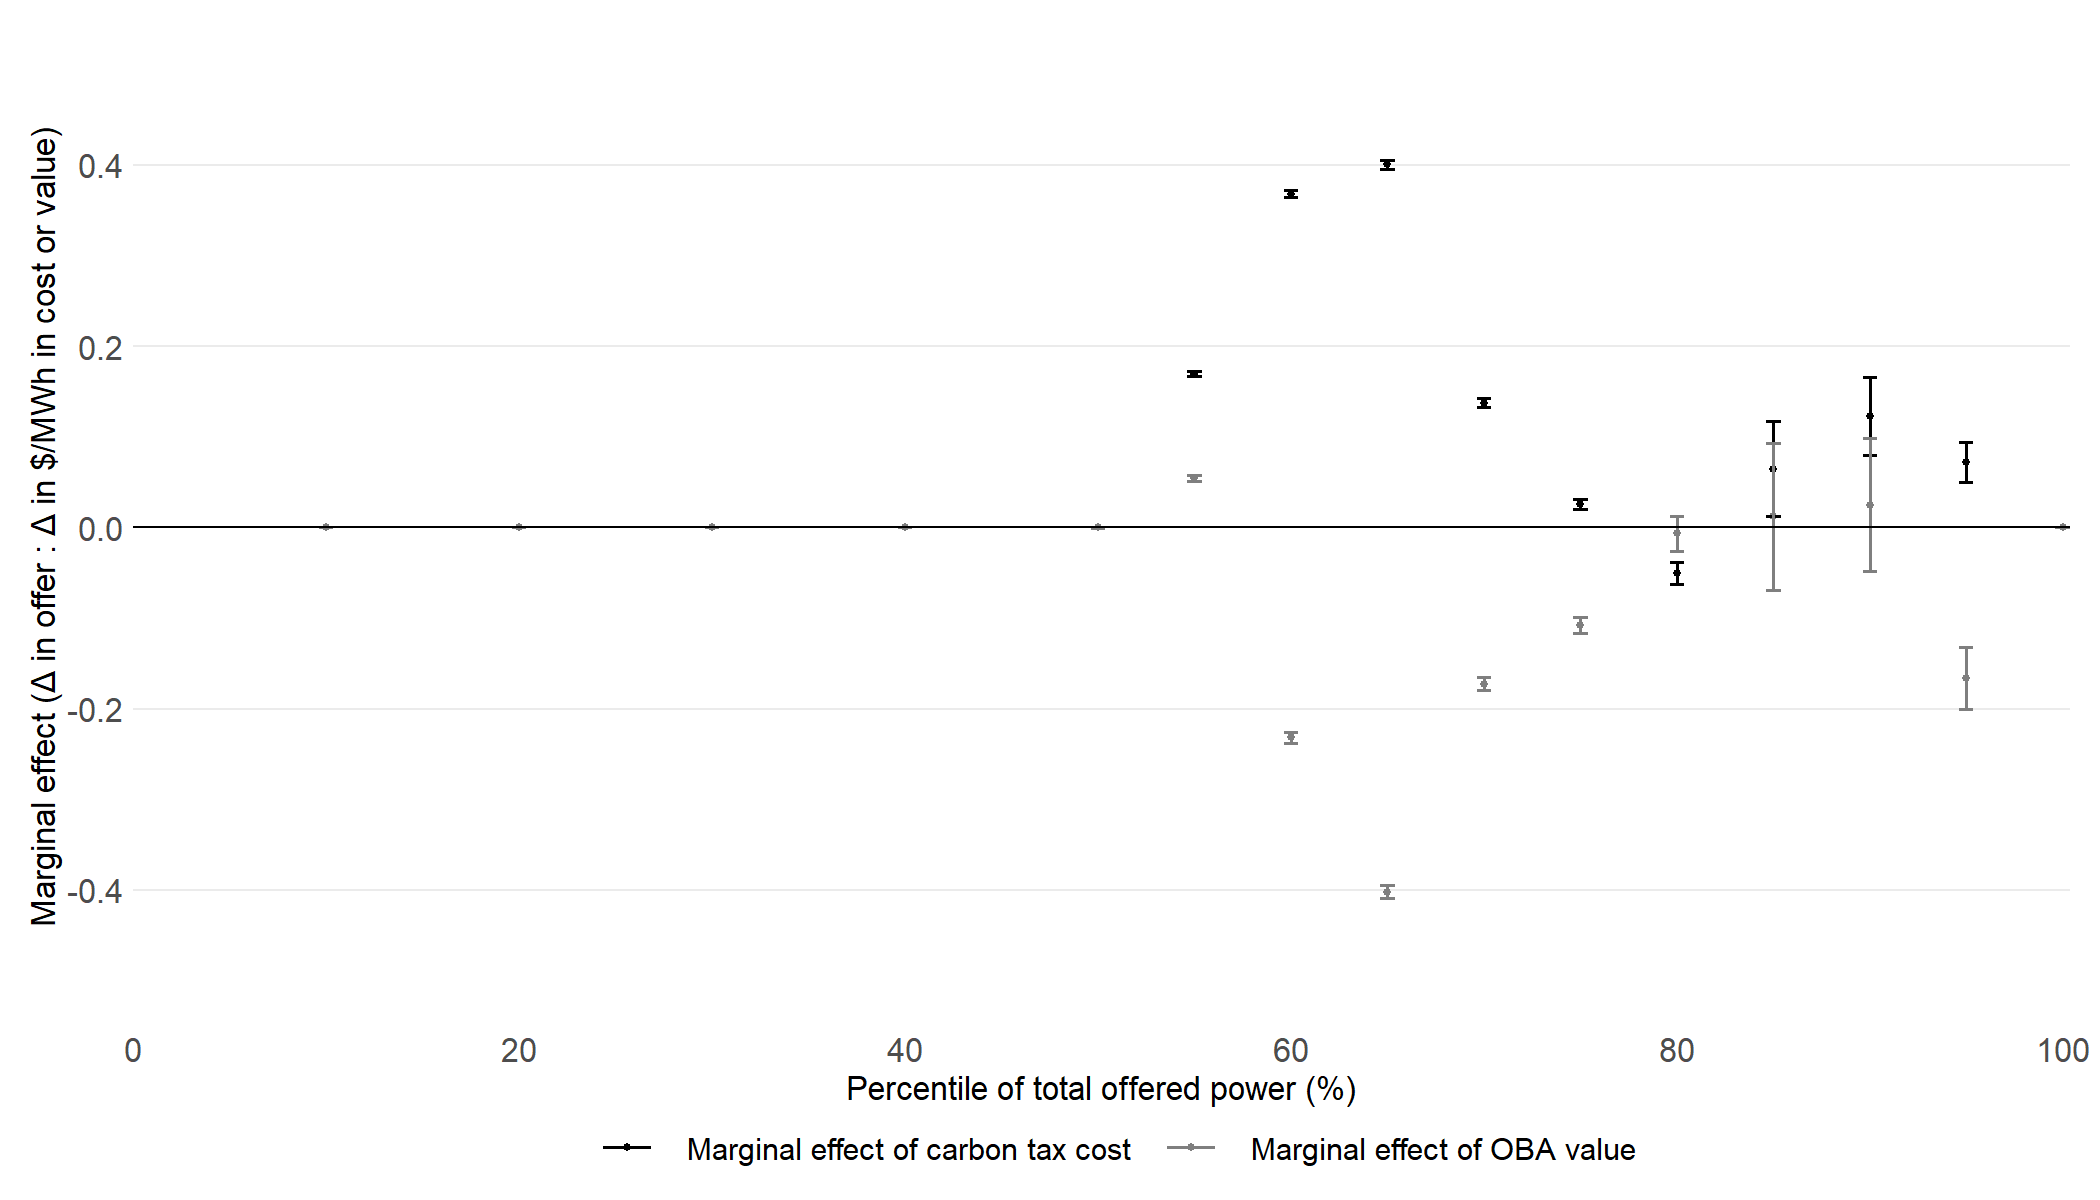
\includegraphics[width=.7\paperwidth]{../images/all_plants_no_peaks.png}}; \vspace{1cm}
   \vfill
\end{frame}

\begin{frame}{Carbon pricing pass through, full market}
   \tikz [remember picture,overlay]
    \node[yshift=-.6cm,xshift=0cm] at (current page.center)
        {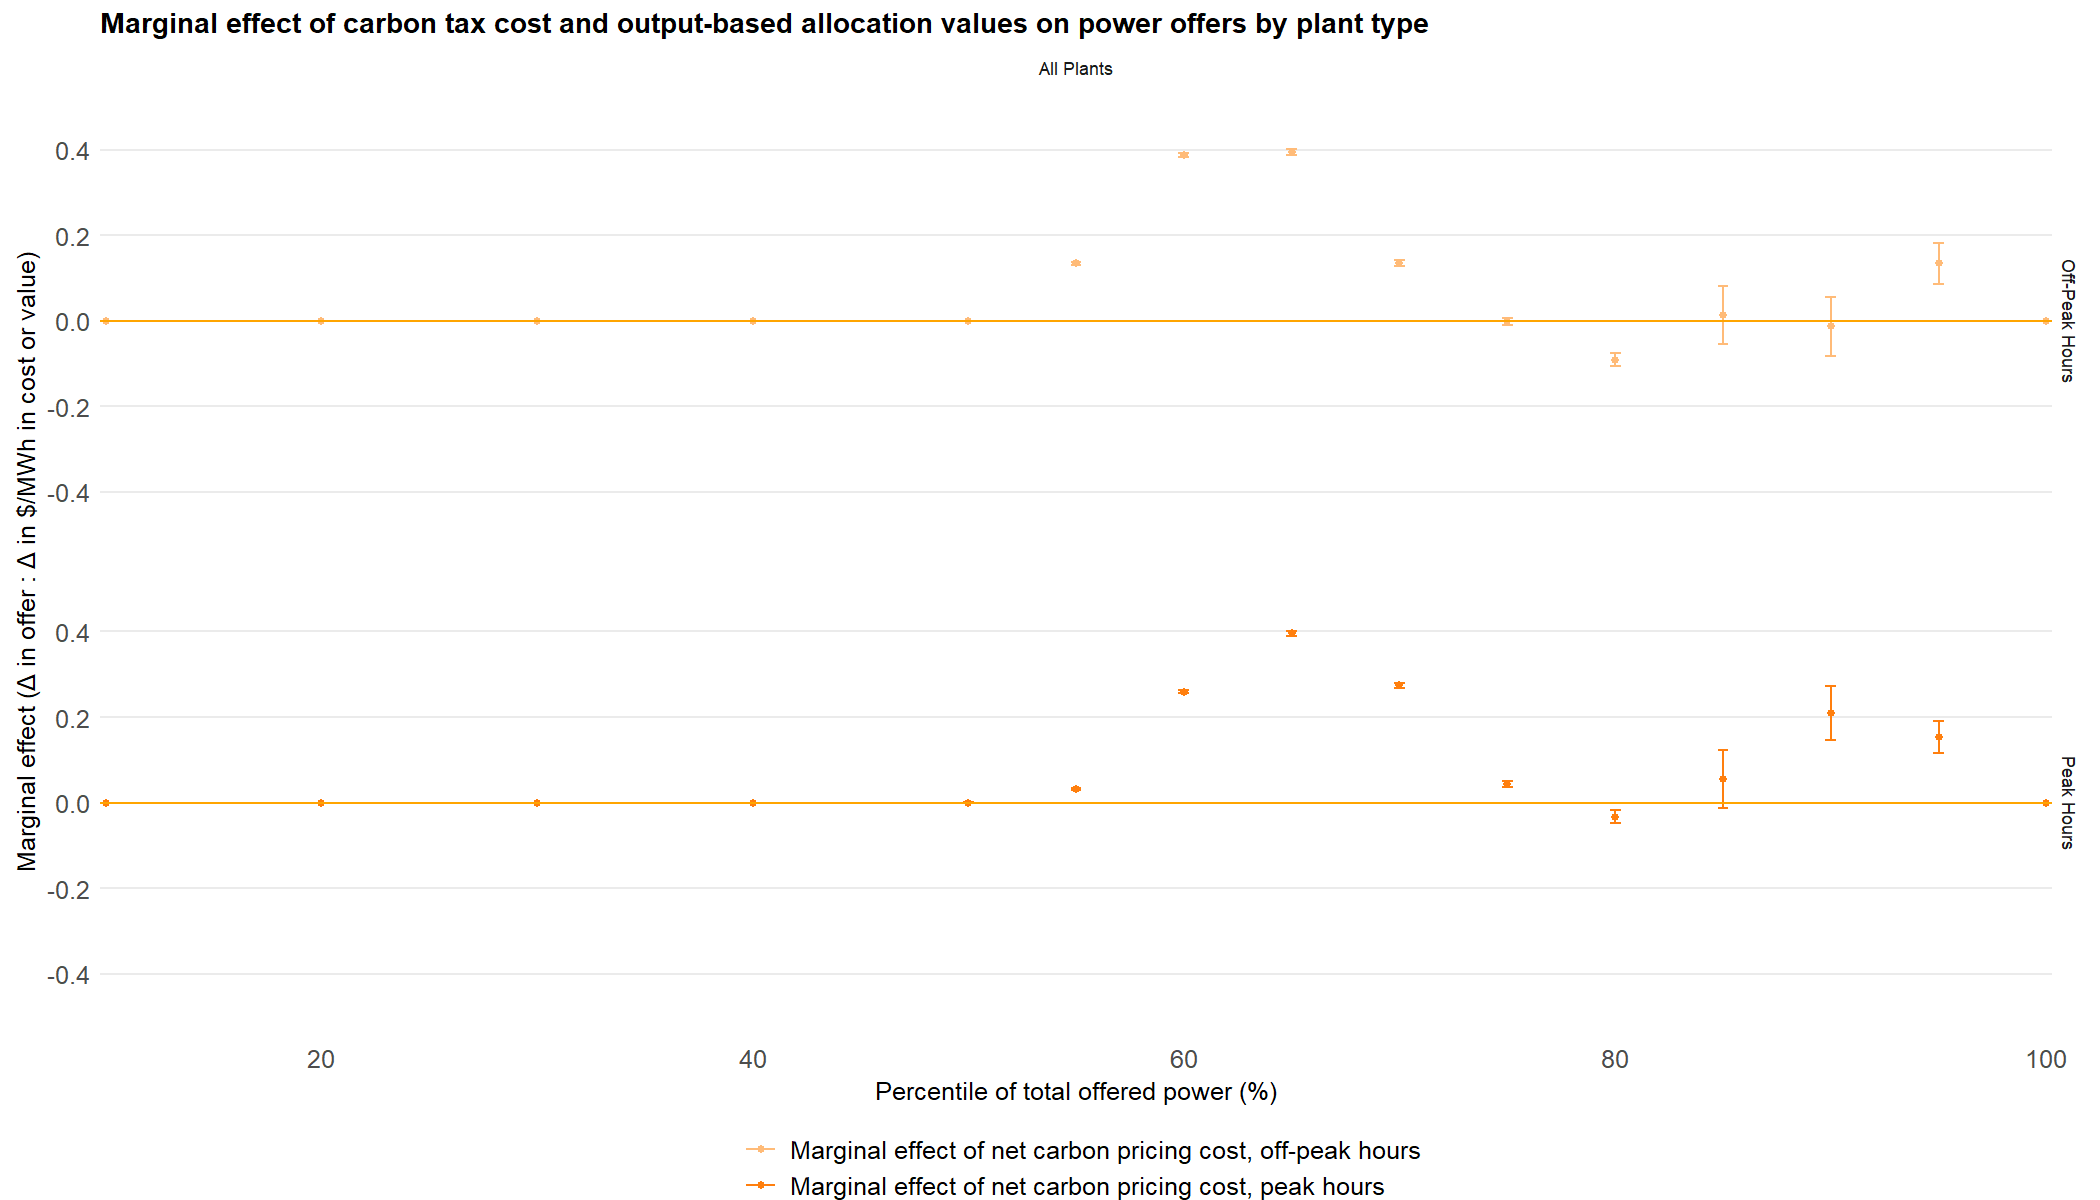
\includegraphics[width=.7\paperwidth]{../images/all_plants_net_peak.png}}; \vspace{1cm}
   \vfill
\end{frame}


\section{Discussion}

\begin{frame}{Discussion}
   \begin{itemize}
   \item Alberta's energy-only power market provides an ideal environment to study carbon price pass-through
    \item Alberta policy changes alter both carbon prices and output-based credit allocations provide facility-specific treatment
    \item Results imply much lower pass-through rates than previous work in this area
    \item The question is why this would be the case?
    \small\begin{itemize}
    \item Coal-to-gas price ratios (Cullen and Mansur (2017))
    \item Strategic behaviour
    \item Omitted variables (facilities with invariant bids)
    \item Changes in ownership and the role of the Balancing Pool during our sample period
    \end{itemize}
     \end{itemize}
   \vfill
\end{frame}



\section{Contact}


%\begin{frame}{Oil sands reserves\hspace{3cm} \small Source: AER (2013)}
%\pgfputat{\pgfxy(0,.25)}{\pgfimage[width=4.25in]{AB_reserves.pdf}}
%\end{frame}

\begin{frame}{Contact information}
\vspace{-.5 cm}
\begin{center}
Andrew Leach, Alberta School of Business, University of Alberta\\[2ex]

\begin{minipage}[t]{0.15\textwidth} % 27.5% of the page width for the first row of icons
	\vspace{-\baselineskip} % Required for vertically aligning minipages
	\end{minipage}
      \hfill
\begin{minipage}[t]{0.5\textwidth} % 27.5% of the page width for the first row of icons
	\vspace{-\baselineskip} % Required for vertically aligning minipages
	%\icon{Phone}{12}{\textcolor[rgb]{0.00,0.00,0.00}{+1 780-492-8489}}\\[-0.5ex]
	\icon{EnvelopeO}{12}{\href{mailto:aleach@ualberta.ca}{aleach@ualberta.ca}}\\[-0.5ex]
    \icon{Globe}{12}{\href{https://aleach.ca}{aleach.ca}}
    \end{minipage}
      \hfill
\begin{minipage}[t]{0.4\textwidth} % 27.5% of the page width for the second row of icons
	\vspace{-\baselineskip} % Required for vertically aligning minipages
	
	% The first parameter is the FontAwesome icon name, the second is the box size and the third is the text
	% Other icons can be found by referring to fontawesome.pdf (supplied with the template) and using the word after \fa in the command for the icon you want
    %\icon{Linkedin}{12}{\href{https://linkedin.com/in/leach-econ}{leach-econ}}\\	[-0.5ex]	
    \icon{Github}{12}{\href{https://github.com/leachandrew}{leachandrew}}\\[-0.5ex]
    \icon{Twitter}{12}{\href{https://twitter.com/andrew_leach}{@andrew\TextUnderscore leach}}
\end{minipage}
\\[+6ex]
Blake Shaffer, Dept of Economics and School of Public Policy, University of Calgary\\[2ex]

\begin{minipage}[t]{0.15\textwidth} % 27.5% of the page width for the first row of icons
	\vspace{-\baselineskip} % Required for vertically aligning minipages
	\end{minipage}
      \hfill
\begin{minipage}[t]{0.5\textwidth} % 27.5% of the page width for the first row of icons
	\vspace{-\baselineskip} % Required for vertically aligning minipages
	\icon{EnvelopeO}{12}{\href{mailto:blake.shaffer@ucalgary.ca}{blake.shaffer@ucalgary.ca}}\\[-0.5ex]
    \icon{Globe}{12}{\href{https://blakeshaffer.ca}{blakeshaffer.ca}}
    \end{minipage}
      \hfill
\begin{minipage}[t]{0.4\textwidth} % 27.5% of the page width for the second row of icons
	\vspace{-\baselineskip} % Required for vertically aligning minipages
	
	% The first parameter is the FontAwesome icon name, the second is the box size and the third is the text
	% Other icons can be found by referring to fontawesome.pdf (supplied with the template) and using the word after \fa in the command for the icon you want
    \icon{Github}{12}{\href{https://github.com/blakeshaffer}{blakeshaffer}}\\[-0.5ex]
    \icon{Twitter}{12}{\href{https://twitter.com/bcshaffer}{@bcshaffer}}
\end{minipage}
\end{center}

\vfill
\end{frame}



\end{document} 